\documentclass{article}

%%%%%%%%%%%%%%%%%%%%%%%%%%%%%%%%%%%%%%%%%%%%%%%%%%%%%%%%
% Packages
%%%%%%%%%%%%%%%%%%%%%%%%%%%%%%%%%%%%%%%%%%%%%%%%%%%%%%%%

%\usepackage[utf8]{inputenc} % for overleaf/PLM
\usepackage[latin1]{inputenc} % averil local
\usepackage[T1]{fontenc} % hyphenation
\usepackage{fullpage} % DO NOT USE IN BEAMER
\usepackage[british,UKenglish,USenglish,american]{babel}
%\usepackage{appendix}
\usepackage{amssymb,amsmath,amsthm,enumerate}
\usepackage{mathtools} % coloneqq
%\usepackage{easybmat}
\usepackage{enumitem}
%\usepackage{tikz}
%\usepackage{caption}
\usepackage{float} % [H]
%\usepackage{bbold}
\usepackage{xcolor}
\usepackage{stmaryrd} % ll/rr brackets
%\usepackage[notcite, notref]{showkeys}
%\usepackage[tworuled,vlined,nofillcomment]{algorithm2e}
\usepackage[ruled,vlined]{algorithm2e}
%\usepackage{cases} % numbered lines in cases (numcases and subnumcases)
\usepackage[overload]{empheq} % source : https://tex.stackexchange.com/questions/31951/separate-labels-in-cases
\usepackage{caption} % to have subfigures
\usepackage{subcaption} % to have subfigures
\usepackage{cleveref} % \cref. 

%%%%%%%%%%%%%%%%%%%%%%%%%%%%%%%%%%%%%%%%%%%%%%%%%%%%%%%%
% Format
%%%%%%%%%%%%%%%%%%%%%%%%%%%%%%%%%%%%%%%%%%%%%%%%%%%%%%%%

\title{Notes on fixed-point procedure}
\author{} 
\date{}

\SetKwRepeat{Do}{do}{while} % for algorithm2e package, add do-while

% set dashes instead of bullets for item lists
\setlist[itemize,1]{label=$-$}
\setlist[itemize,2]{label=$-$}
\setlist[itemize,3]{label=$-$}

% remove unnecessary formatting of clever references
\crefdefaultlabelformat{(#2#1#3)}
\crefname{equation}{}{}

%%%%%%%%%%%%%%%%%%%%%%%%%%%%%%%%%%%%%%%%%%%%%%%%%%%%%%%%
% Theorems
%%%%%%%%%%%%%%%%%%%%%%%%%%%%%%%%%%%%%%%%%%%%%%%%%%%%%%%%

\newtheorem{proposition}{Proposition}[section]
\newtheorem{definition}{Definition}[section]
\newtheorem{theoreme}{Theorem}[section]
\newtheorem{remarque}{Remark}[section]
\newtheorem{lemme}{Lemma}[section]
\numberwithin{equation}{section}

%%%%%%%%%%%%%%%%%%%%%%%%%%%%%%%%%%%%%%%%%%%%%%%%%%%%%%%%
% Commands
%%%%%%%%%%%%%%%%%%%%%%%%%%%%%%%%%%%%%%%%%%%%%%%%%%%%%%%%

\newcommand{\N}{\mathbb{N}}
\newcommand{\Z}{\mathbb{Z}}
\newcommand{\R}{\mathbb{R}}
\newcommand{\lp}{\left(}
\newcommand{\rp}{\right)}
\newcommand{\tran}[1]{\prescript{t}{}{#1}}
\newcommand{\vol}{\textup{Vol}}
\newcommand{\red}{\textcolor{red}}
\newcommand{\blue}{\textcolor{blue}}

\newcommand{\todo}[1]{{\color{red}\textbf{#1}}}
\newcommand{\vv}[1]{\begin{pmatrix} #1 \end{pmatrix}} % vector
\newcommand{\mysubeq}[2]{ % first argument : label, second : align content
	\begin{subequations}\label{#1}
		\begin{align}[left = {\empheqlbrace}]
			#2
		\end{align}
	\end{subequations}	
}
\newcommand{\mysubcaption}[1]{
	\vspace*{5pt}
	\begin{minipage}{0.8\linewidth}
		\begin{center}
			\footnotesize\emph{#1}
		\end{center}
	\end{minipage}
}
\newcommand{\imh}{\textwidth} % meant to be redefined locally

%\renewcommand\appendixpagename{Appendix}
%\renewcommand\appendixtocname{Appendix}
\renewcommand{\qedsymbol}{$\blacksquare$}

% local vocabulary
\newcommand{\ve}{{\overline{v}_e}} % bound on the speed in the support of fe
\newcommand{\we}{{\underline{w}_e}} % transformation of \ve
\newcommand{\DomUpL}{{\mathcal{D}_1}} % domain over the critical char, x=0 side
\newcommand{\DomUpR}{{\mathcal{D}_2}} % domain over the critical char, x=1 side
\newcommand{\DomLow}{{\mathcal{D}_3}} % domain under the critical char + over -\ve
\newcommand{\IntUpL}{{\mathcal{I}_1}} % part of n_i on \DomUpL
\newcommand{\IntUpR}{{\mathcal{I}_2}} % part of n_i on \DomUpR
\newcommand{\IntLow}{{\mathcal{I}_3}} % part of n_i on \DomLow
\newcommand{\domfel}{{\underline{v}}} % lower bound on a segment on which fe >=  \minfe
\newcommand{\domfeu}{{\overline{v}}} % upper bound on a segment on which fe >=  \minfe
\newcommand{\minfe}{{\underline{c}}} % lower bound on f_e on a segment [-\domfeu, -\domfel]
\newcommand{\maxfe}{{\overline{c}}} % upper bound on f_e

%%%%%%%%%%%%%%%%%%%%%%%%%%%%%%%%%%%%%%%%%%%%%%%%%%%%%%%%
%%%%%%%%%%%%%%%%%%%%%%%%%%%%%%%%%%%%%%%%%%%%%%%%%%%%%%%%
%%%%%%%%%%%%%%%%%%%%%%%%%%%%%%%%%%%%%%%%%%%%%%%%%%%%%%%%

\begin{document}

\maketitle

%Let us define for all $0 < \alpha \leqslant \beta$ the set
%\begin{align*}
%	\mathcal{K}^{\alpha,\beta} \coloneqq \left\{\varphi \in \mathcal{C}^2\left([0,1], \mathbb{R}^{-}\right) \ |\ \varphi(0) = \varphi'(0) = 0, \quad - \beta \leqslant \varphi'' \leqslant - \alpha. \right\}
%\end{align*}
%
%\paragraph{Estimates on the set $\mathcal{K}$}
%
%Since $\varphi : [0,1] \mapsto \mathbb{R}^-$ is decreasing, its inverse $\varphi^{-1} : \mathbb{R}^- \mapsto [0,1]$ is well-defined. By integration and using $\left(\varphi^{-1}\right)' = (\varphi'\circ \varphi^{-1})^{-1}$, we have
%\mysubeq{eq:convex_bounds}{
%	- \beta x &\leqslant \varphi'(x) \leqslant - \alpha x \label{eq:convex_bounds_phiprime} \\
%	- \beta \frac{x^2}{2} &\leqslant \varphi(x) \leqslant - \alpha \frac{x^2}{2} \label{eq:convex_bounds_phi} \\
%	\sqrt{-\frac{2y}{\beta}} &\leqslant \varphi^{-1}(y) \leqslant \sqrt{-\frac{2y}{\alpha}} \label{eq:convex_bounds_phiinv} \\
%	\frac{-1}{\alpha\sqrt{-\frac{2y}{\beta}}} &\leqslant (\varphi^{-1})'(y) \leqslant \frac{-1}{\beta\sqrt{-\frac{2y}{\alpha}}} \label{eq:convex_bounds_phiinv} 
%}

\tableofcontents

% TO WRITE
% What are the characteristics equations
% The choice of the domain $v\leqslant0$ and $x\in[0,1]$
% Symmetries

\section{Estimates}

\subsection{Upper bounds on the densities}

We want to obtain estimates on $n_i - n_e$. We make the following assumptions:
\begin{itemize}
\item The electron density $f_e$ satisfies the boundary condition, and is bounded by a constant $\maxfe \geqslant 0$. 
\item The potential $\varphi$ is strongly concave, i.e. there exists $\alpha>0$ such that $\varphi''(x) \leqslant - \alpha$ uniformly over $x\in[0,1]$.
\item We have $\varphi(0) = \varphi'(0) = 0$.
\end{itemize}
The assumptions on $\varphi$ yield that
\begin{align}\label{eq:phi_concave_consequences}
	\varphi'(x) \leqslant- \alpha x, \quad \varphi(x) \leqslant - \alpha \frac{x^2}{2}.
\end{align}

Let us first focus on $n_e(x)$. The characteristics of the electron density are the level lines of
\begin{align}\label{eq:def_Le}
	\mathcal{L}_e(x,v) \coloneqq \frac{v^2}{2} - \frac{1}{\mu} \varphi(x).
\end{align}
Since $\varphi$ is strongly concave, these curves are closed. Since $f_e$ satisfies the homogeneous boundary condition, its support is embedded in $\left\{(x,v) \ |\ \frac{v^2}{2} - \frac{1}{\mu} \varphi(x) \leqslant \frac{0^2}{2} - \frac{1}{\mu} \varphi(1)\right\}$. In particular, we denote by $\ve$ the extremal speed of the support, given by
\begin{align}\label{eq:def_ve}
	\ve \coloneqq \sqrt{-\frac{2}{\mu} \varphi(1)}.
\end{align}
We can roughly majorize
\begin{align*}
	n_e(x) = \int_{v\in\mathbb{R}} f_e(x,v) dv \leqslant \int_{v=-\ve}^{\ve} \maxfe dv = 2 \maxfe \ve \leqslant 2 \maxfe \sqrt{-\frac{2}{\mu} \varphi(1)}.
\end{align*}

The estimates on $n_i$ are slightly more technical. Let the ion Lyapunov function be defined as
\begin{align}\label{eq:def_Li}
	\mathcal{L}_i(x,v) \coloneqq \frac{v^2}{2} + \varphi(x).
\end{align}
In the sequel, we will heavily rely on the level lines of $\mathcal{L}_i$ to partition the space. We distinguish the \emph{critical characteristic} as the curve $\left\{\mathcal{L}_i = 0\right\}$.
Let $x\in[0,1]$ and $v \in \mathbb{R}_{-}$. We denote by $(x_b(x,v),v_b(x,v))$ the intersection of the boundary $\left\{x=0\right\}\cap\left\{v=0\right\}$ with the characteristic issued from $(x,v)$, equal to
\begin{align*}
	\vv{x_b(x,v) \\ v_b(x,v)} \coloneqq 
	\begin{cases}
		\vv{\varphi^{-1}\left(\frac{v^2}{2} + \varphi(x)\right) \\ 0} & \text{if } \mathcal{L}_i(x,v) \leqslant 0, \\
		\vv{0 \\ - \sqrt{\frac{v^2}{2} + \varphi(x)}} & \text{if } \mathcal{L}_i(x,v) > 0.
	\end{cases}
\end{align*}
In the following paragraph, we use $(x(t),v(t))_{t\leqslant0}$ to denote the characteristic reaching $(x_b(x,v),v_b(x,v))$ at $t=0$. 
We use the symmetry of $f_i$ to write 
\begin{align*}
	n_i(x) = 2 \int_{v\in\mathbb{R}^{-}} f_i(x_b(x,v), v_b(x,v)) dv = 2 \int_{v\in\mathbb{R}^{-}}\int_{t=-\infty}^{0} f_e(x(t),v(t)) dt dv.
\end{align*}
The lower bound $t \to -\infty$ is artificial, since the characteristic exits the support of $f_e$ in finite time. We will split the double integral in three domains, represented in \cref{fig:charmaps_domainmap}:
\begin{enumerate}
\item $\DomUpL$ will be $\left\{(v,t) \in \mathbb{R}_{-}^2 \ |\ \mathcal{L}_i(x,v) \leqslant 0 \text{ and } x(t) \leqslant x \right\}$. This is the region contained between the $x-$axis, the critical characteristic and the vertical line going through $x$.
\item $\DomUpR$ is $\left\{(v,t) \in \mathbb{R}_{-}^2 \ |\ \mathcal{L}_i(x,v) \leqslant 0 \text{ and } x < x(t) \leqslant 1 \right\}$. It cover the part of the domain intersecting $\left\{\mathcal{L}_i \leqslant 0\right\} \setminus \DomUpL$.
\item $\DomLow$ is defined by $\left\{(v,t) \in \mathbb{R}_{-}^2 \ |\ \mathcal{L}_i(x,v) > 0 \text{ and } -\ve \leqslant v(t) \right\}$. 
\end{enumerate}

\begin{figure}
	\centering
	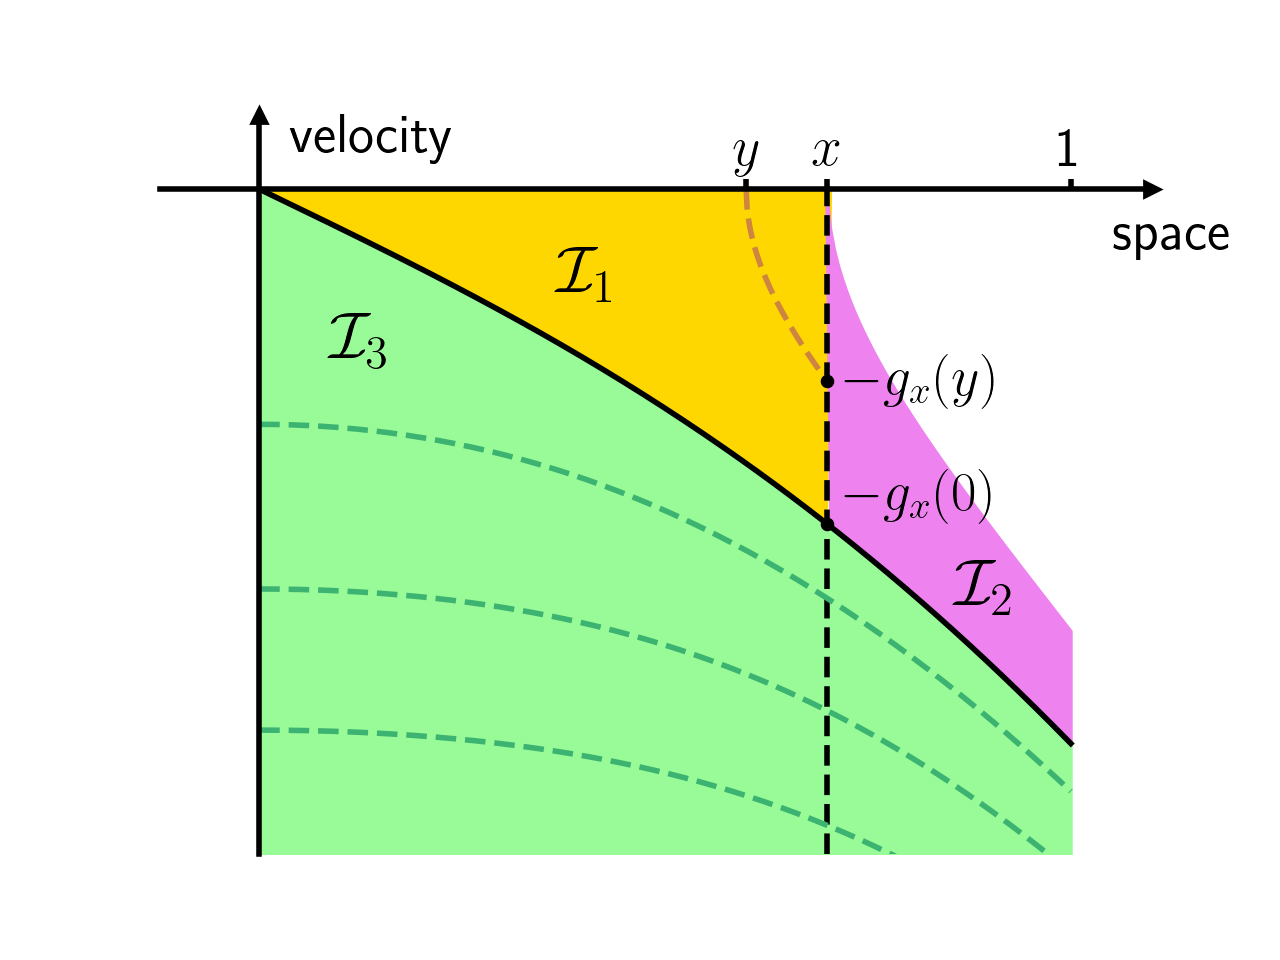
\includegraphics[width=0.5\linewidth]{images/fpcharmaps_domainmap}
	\caption{Partition of $\mathbb{R}_{-}^2$.}
	\label{fig:charmaps_domainmap}
\end{figure}

Since $f_e(x(t),v(t))$ vanishes outside $\DomUpL \cup \DomUpR \cup \DomLow$, we may exactly decompose $n_i$ in 
\begin{align*}
	\frac{n_i(x)}{2} = \underbrace{\iint_{(v,t) \in \DomUpL} f_e(x(t),v(t)) dt dv}_{\IntUpL} + \underbrace{\iint_{(v,t) \in \DomUpR} f_e(x(t),v(t)) dt dv}_{\IntUpR} + \underbrace{\iint_{(v,t) \in \DomLow} f_e(x(t),v(t)) dt dv}_{\IntLow} 
\end{align*}

Each term will be bound separately. 

\paragraph{Bound on $\IntUpL$}

Let $v_0(x) \coloneqq \sqrt{-2\varphi(x)}$ be the velocity such that $(x, -v_0(x))$ belongs to the critical characteristic. 
The characteristics in the domain $\DomUpL$ are joining points $(x,v)$, with $v \in [-v_0(x),0]$, with points $(x_b(x,v), 0)$. Therefore, we may use the reparametrization 
\begin{align*}
	y = x(t), \quad dy = \dot{x}(t) dt = v(t) dt = - \left(v^2 + 2 \left(\varphi(x) - \varphi(x(t))\right)\right)^{1/2} dt = - \left(v^2 + 2 \left(\varphi(x) - \varphi(y)\right)\right)^{1/2} dt	
\end{align*}
The integral $\IntUpL$ becomes
\begin{align*}
	\IntUpL = \int_{v=-v_0(x)}^0 \int_{y=x}^{x_b(x,v)} f_e(y,- \left(v^2 + 2 \left(\varphi(x) - \varphi(y)\right)\right)^{1/2}) \frac{-1}{\left(v^2 + 2 \left(\varphi(x) - \varphi(y)\right)\right)^{1/2}} dy dv.
\end{align*}
By exchanging the bounds of the integrals along $y$, and using $f_e \leqslant \maxfe$, we get
\begin{align*}
	\IntUpL \leqslant \maxfe \int_{v=-v_0(x)}^0 \int_{y=x_b(x,v)}^{x} \frac{1}{\left(v^2 + 2 \left(\varphi(x) - \varphi(y)\right)\right)^{1/2}} dy dv.
\end{align*}
In order to use the explicit $v^2$, we use Fubini theorem to switch the order of integration (since everything is positive). To do this, we write
\begin{align*}
	\begin{cases}
		- v_0(x) \leqslant v \leqslant 0 \\
		x_b(x,v) \leqslant y \leqslant x 
	\end{cases}
	\quad \iff \quad 
	\begin{cases}
		0 \leqslant y \leqslant x \\
		- v_0(x) \leqslant v \leqslant - g_x(y)
	\end{cases}
\end{align*}
where $y = x_b(x,v) = \varphi^{-1}\left(\frac{v^2}{2} + \varphi(x)\right)$ is equivalent to $v = - g_x(y) \coloneqq - \left(2\left(\varphi(y) - \varphi(x)\right)\right)^{1/2}$. In the sequel, we drop the $x$ and simply write $g(y)$. The function $g : [0,x] \mapsto \mathbb{R}^{+}$ is well-defined, since $y \leqslant x \implies \varphi(y) \geqslant \varphi(x)$. By the assumption of strong concavity of $\varphi$, $g$ is positive whenever $y < x$. Finally, using that $v_0(x) = g(0)$, may now write 
\begin{align*}
	\IntUpL \leqslant \maxfe \int_{y=0}^{x} \int_{v=-v_0(x)}^{-g(y)}  \frac{1}{\left(v^2 - g^2(y)\right)^{1/2}} dv dy \underset{\text{with }w\coloneqq g(y)-v}{=} \maxfe \int_{y=0}^{x} \int_{w=0}^{g(0)-g(y)}  \frac{1}{\left(w^2 + 2 w g(y)\right)^{1/2}} dv dy.
\end{align*}
By integration with $\frac{d}{dy} [\sinh^{-1}\left(\sqrt{\frac{y}{a}}\right)] = \frac{1}{(y^2 + 2 a y)^{1/2}}$, we obtain
\begin{align*}
	\IntUpL \leqslant \maxfe \int_{y=0}^{x} \left[\sinh^{-1}\left(\sqrt{\frac{v}{g(y)}}\right)\right]^{g(0)-g(y)}_{0} dv = \maxfe \int_{y=0}^{x} \sinh^{-1}\left(\sqrt{\frac{g(0)-g(y)}{g(y)}}\right) dv.
\end{align*}
We use the coarse estimates $\sinh^{-1}(z) \leqslant z$ and $\sqrt{\frac{a-b}{b}} \leqslant \sqrt{\frac{a}{b}}$ to reduce the expression to
\begin{align*}
	\IntUpL \leqslant \maxfe \sqrt{g(0)} \int_{y=0}^{x} \frac{1}{\sqrt{g(y)}} dv = \maxfe \sqrt{g(0)} \int_{y=0}^{x} \frac{1}{\left(2\left(\varphi(y) - \varphi(x)\right)\right)^{1/4}} dv.
\end{align*}
Using the strong concavity of $\varphi$, and the sign $-\varphi'(y) \geqslant 0$, we get
\begin{align*}
	\varphi(y) - \varphi(x) \geqslant \frac{\alpha}{2} |x - y|^2 - \varphi'(y)(x-y) \geqslant \frac{\alpha}{2} (x - y)^2.
\end{align*}
With this, we may finally write
\begin{align*}
	\IntUpL \leqslant \maxfe \sqrt{g(0)} \int_{y=0}^{x} \frac{1}{\alpha^{1/4}\left(x-y\right)^{1/2}} dv = \frac{2 \maxfe}{\alpha^{1/4}} \sqrt{g(0) x} = \frac{2 \maxfe}{\alpha^{1/4}} \sqrt{\sqrt{-2\varphi(x)} x} \leqslant \frac{2 \maxfe}{\alpha^{1/4}} \left(-2\varphi(1)\right)^{1/4}.
\end{align*}

\paragraph{Bound on $\IntUpR$}

We use the same reparametrization as for $\IntUpR$, but with $y \in [x,1]$, to obtain
\begin{align*}
	\IntUpR \leqslant \maxfe \int_{v=-v_0(x)}^{0} \int_{y=x}^{1} \frac{1}{\left(v^2 + 2(\varphi(x) - \varphi(y))\right)^{1/2}} dy dv.
\end{align*}
On $y \geqslant x$, we may directly use
\begin{align*}
	\varphi(x) - \varphi(y) \geqslant \frac{\alpha}{2} |y - x|^2 - \varphi'(x) (y-x) \geqslant \frac{\alpha}{2} (y - x)^2
\end{align*}
to get
\begin{align*}
	\IntUpR \leqslant \maxfe \int_{v=-v_0(x)}^{0} \int_{y=x}^{1} \frac{1}{\left(v^2 + \alpha(y-x)^2\right)^{1/2}} dy dv \leqslant \maxfe \max\left(1,\frac{1}{\sqrt{\alpha}}\right) \int_{v=0}^{v_0(x)} \int_{z=0}^{1-x} \frac{1}{\left(v^2 + z^2\right)^{1/2}} dy dv.
\end{align*}
By switching to polar coordinates over the (larger) domain $(\theta,r) \in [0,\frac{\pi}{2}] \times [0,\sqrt{v_0(x)^2 + (1-x)^2}]$, we conclude to 
\begin{align*}
	\IntUpR \leqslant \maxfe \max\left(1,\frac{1}{\sqrt{\alpha}}\right) \frac{\pi}{2} \sqrt{v_0(x)^2 + (1-x)^2} \leqslant \maxfe \max\left(1,\frac{1}{\sqrt{\alpha}}\right) \frac{\pi}{2} \sqrt{1 - 2\varphi(1)}.
\end{align*} 

\paragraph{Bound on $\IntLow$}

The domain $\DomLow$ is covered by characteristics linking $x=1$ to $x=0$. We may use the same reparametrization within fixed bounds over $y$:
\begin{align*}
	\IntLow \leqslant \maxfe \int_{v=-\ve}^{-v_0(x)} \int_{y=0}^{1} \frac{1}{\left(v^2 + 2 \left(\varphi(x) - \varphi(y)\right)\right)^{1/2}} dy dv = \maxfe \int_{y=0}^{1} \int_{v=-\ve}^{-v_0(x)} \frac{1}{\left(v^2 + 2 \left(\varphi(x) - \varphi(y)\right)\right)^{1/2}} dy dv.
\end{align*}
We will use the same argument as for $\IntUpR$, but with characteristics ending on $x=0$ instead of $x=x$. Our first step is then to replace $v$ by $w$ the velocity at $x=0$, defined by $\frac{v^2}{2} + \varphi(x) = \frac{w^2}{2} + 0$. We have
\begin{align*}
	 w = - \left(v^2 + 2 \varphi(x)\right)^{1/2} \in [-\we, 0], \quad v = - \left(v^2 - 2 \varphi(x)\right)^{1/2}, \quad dv = \frac{-w}{\left(w^2-2\varphi(x)\right)^{1/2}} dw,
\end{align*}
where $\we \coloneqq \left(\ve^2 + 2 \varphi(x)\right)^{1/2} \leqslant \ve \leqslant \sqrt{-2\varphi(1)}$. Using the estimate $-\varphi(y) \geqslant \alpha \frac{y^2}{2}$, we conclude similarly that
\begin{align*}
	\IntLow 
	\leqslant \maxfe \int_{y=0}^{1} \int_{w=-\we}^{0} \frac{1}{\left(w^2 - 2\varphi(y)\right)^{1/2}} dy dv 
	= \maxfe \int_{y=0}^{1} \int_{w=0}^{\we} \frac{1}{\left(w^2 + \alpha y^2\right)^{1/2}} dy dv
	\leqslant \maxfe \max\left(1,\frac{1}{\sqrt{\alpha}}\right) \frac{\pi}{2} \sqrt{1 - 2 \varphi(1)}.
\end{align*}

In conclusion, we obtained the uniform bound
\begin{align*}
	n_i(x) \leqslant \frac{4}{\alpha^{1/4}} \left(-2\varphi(1)\right)^{1/4} + 4 \maxfe \max\left(1,\frac{1}{\sqrt{\alpha}}\right) \frac{\pi}{2} \sqrt{1 - 2 \varphi(1)}.
\end{align*}

\subsection{Lower bound on $n_i$}

Let us consider that $f_{e,b}$ is positive on a segment. More precisely, we assume that there exists $0 \leqslant \domfel < \domfeu \leqslant \ve$ and $\minfe > 0$ such that $f_e([-\domfeu,-\domfel]) \geqslant \minfe$.
The value $\minfe$ is propagated along every electron characteristic crossing $(x=0,v\in[-\domfeu,-\domfel])$, so that we may use the lower estimate
\begin{align*}
	f_e(x,v) \geqslant \minfe \,\textbf{1}_{\left\{\mathcal{L}_e(0,\domfel) \leqslant \mathcal{L}_e(x,v) \leqslant \mathcal{L}_e(0,\domfeu)\right\}}.
\end{align*}
Let us parametrize the electron characteristic issued from $(0,-\domfeu)$ by $(\overline{y}(v), v)$, with $v\in[-\domfeu,0]$. Let $x\in[0,1]$, and define $\underline{w}$ and $\overline{w}$ by
\begin{align*}
	\begin{cases}
		\mathcal{L}_i(0,-\domfeu) = \mathcal{L}_i(x,-\underline{w}), \\
		\mathcal{L}_i(0,-\domfel) = \mathcal{L}_i(x,-\overline{w})
	\end{cases}
	\quad \text{that is} \quad
	\begin{cases}
		\underline{w} \coloneqq \left(\frac{\domfeu^2}{2} - 2 \varphi(x)\right)^{1/2} \\
		\overline{w} \coloneqq \left(\frac{\domfel^2}{2} - 2 \varphi(x)\right)^{1/2}
	\end{cases}
\end{align*}

\begin{figure}
	\centering
	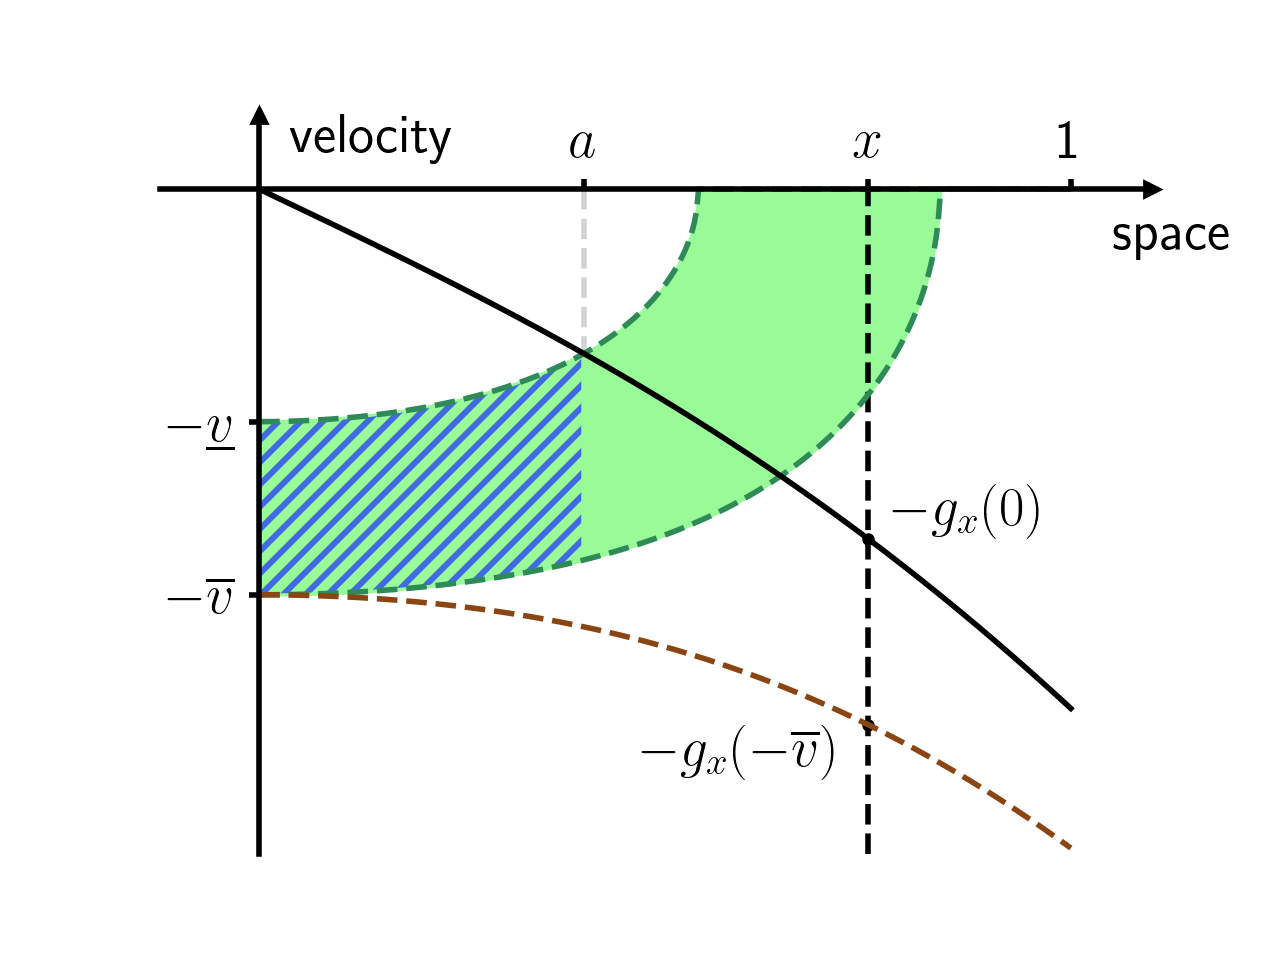
\includegraphics[width=0.5\linewidth]{images/fpcharmaps_lowerboundni}
	\caption{Notations for the lower bound on $n_i$.}
	\mysubcaption{The coloured area corresponds to the domain $\mathcal{L}_e(0,\domfel) \leqslant \mathcal{L}_e(x,v) \leqslant \mathcal{L}_e(0,\domfeu)$, on which we know that $f_e \geqslant \minfe$. The parametrization $(\overline{y}(w),w)$ of the electron characteristic crossing $(0,-\domfeu)$ is equivalent to $(y,-h(y))$.}
	\label{fig:charmaps_lowerboundni}
\end{figure}

Then, using the (now classical) reparametrization, the ion density satisfies
\begin{align*}
	n_i(x) \geqslant \minfe \int_{w=-\overline{w}}^{-\underline{w}} \int_{y=0}^{\overline{y}(w)} \frac{1}{\left(w^2 + 2\left(\varphi(x) - \varphi(y)\right)\right)^{1/2}} dy dw.
\end{align*}
As for the integral $\IntLow$, we wish to use the velocity at $x=0$ instead of $x=x$. We define $v\in[-\domfeu,-\domfel]$ by
\begin{align*}
	\mathcal{L}_i(0,v) = \mathcal{L}_i(x,w), \quad w = - \left(v^2 - 2 \varphi(x)\right)^{1/2}, \quad dw = \frac{- v}{\left(v^2 - 2 \varphi(x)\right)^{1/2}}.
\end{align*}
This yields
\begin{align*}
	n_i(x) \geqslant \minfe \int_{v=-\domfeu}^{-\domfel} \int_{y=0}^{\overline{y}(w(v))} \frac{1}{\left(v^2 - 2\varphi(y)\right)^{1/2}} dy  \frac{-v}{\left(v^2 - 2 \varphi(x)\right)^{1/2}} dv.
\end{align*}
The upper bound $\overline{y}(w(v))$ is equal to $\varphi^{-1}\left(\frac{\mu}{2}\left(v^2 - \domfeu^2\right)\right)$.
Since $-\varphi(z) \leqslant -\varphi(1)$ for all $z$, this gives
\begin{align*}
	n_i(x) \geqslant \minfe \int_{v=-\domfeu}^{-\domfel} \overline{y}(w(v)) \frac{-v}{v^2 - 2\varphi(1)} dv = \minfe \int_{v=-\domfeu}^{-\domfel} \varphi^{-1}\left(\frac{\mu}{2}\left(v^2 - \domfeu^2\right)\right) \frac{-v}{v^2 - 2\varphi(1)} dv.
\end{align*}

Let $v_* \in ]\domfel,\domfeu[$ be the velocity such that $v_*^2 - \domfel^2 = \frac{\domfeu^2 - \domfel^2}{2}$. We split the integral on $[-\domfeu,-v_*[ \cup [-v_*,\domfel]$ and use the decreasing monotonicity of $\varphi^{-1}$ to write
\begin{align*}
	n_i(x) 
	&\geqslant 0 + \varphi^{-1}\left(\frac{\mu}{2}\left(v_*^2 - \domfeu^2\right)\right) \minfe \int_{v=-v_*}^{-\domfel} \frac{-v}{v^2 - 2\varphi(1)} dv \\
	&= \frac{\minfe}{2} \varphi^{-1}\left(\frac{\mu}{4}\left(\domfel^2 - \domfeu^2\right)\right) \log\left(\frac{v_*^2 - 2 \varphi(1)}{\domfel^2 - 2 \varphi(1)}\right) \\
	&\geqslant \frac{\minfe}{2} \varphi^{-1}\left(\frac{\mu}{4}\left(\domfel^2 - \domfeu^2\right)\right) \log\left(1 + \frac{\domfeu^2 - \domfel^2}{\domfel^2 - 2 \varphi(1)}\right).
\end{align*}



%Using Fubini's theorem, we may rewrite this as
%\begin{align*}
%	n_i(x) \geqslant \minfe  \int_{y=0}^{\overline{y}(-\domfel)} \int_{w=-\overline{w}}^{-h(y)} \frac{1}{\left(w^2 + 2\left(\varphi(x) - \varphi(y)\right)\right)^{1/2}} dw dy,
%\end{align*}
%where $y = \overline{y}(w) \coloneqq \varphi^{-1}\left(\mu \frac{w^2}{2} - \mu \frac{\domfeu^2}{2}\right)^{1/2}$ is equivalent to $w = - h(y) \coloneqq -\left(\domfeu^2 + \frac{2}{\mu} \varphi(y)\right)^{1/2}$.


%\bibliographystyle{alpha}
%\bibliography{CEMRACS.bib}

\end{document}